\documentclass[tikz]{standalone}

\usepackage{amsmath}
\usepackage{unicode-math}
\usepackage{mathtools}
\usepackage{derivative}

\setmainfont{Stix Two Text}
\setmathfont{Stix Two Math}

\usetikzlibrary{arrows.meta,fit,positioning}

\renewcommand{\familydefault}{\sfdefault}

% prefix equation numbers with section number
\numberwithin{equation}{section}

\DeclarePairedDelimiter{\ceil}{\lceil}{\rceil}
\DeclarePairedDelimiter{\floor}{\lfloor}{\rfloor}
\DeclarePairedDelimiter{\abs}{\lvert}{\rvert}
\DeclarePairedDelimiter{\norm}{\lVert}{\rVert}
\DeclarePairedDelimiter{\bra}{\langle}{\rvert}
\DeclarePairedDelimiter{\ket}{\lvert}{\rangle}
\DeclarePairedDelimiter{\expval}{\langle}{\rangle}
\DeclarePairedDelimiter{\norder}{\mathcolon}{\mathcolon}
\DeclarePairedDelimiter{\anorder}{\typecolon}{\typecolon}
	
\newcommand{\laplace}{\mbfnabla^2}
\newcommand{\trans}{{\scriptscriptstyle\mathsf{T}}}

\newcommand{\vdot}{\cdot}
\newcommand{\vcross}{\vectimes}
\newcommand{\vb}[1]{\symbfup{#1}}
\newcommand{\vu}[1]{\hat{\vb{#1}}}
\newcommand*\dd[2][\relax]{\mathop{\ifx\relax#1\odif{#2}\else \odif[order={#1}]{#2}\fi\,}}

\newcommand{\vacuum}{\ket*{\vb{0}}}

\DeclareMathOperator{\trace}{Tr}
\DeclareMathOperator{\sinc}{sinc}

\AtBeginDocument{
	\let\Re\relax
	\let\Im\relax
	\DeclareMathOperator{\Re}{Re}
	\DeclareMathOperator{\Im}{Im}

	\renewcommand{\div}{\mathop{\mbfnabla\vdot}}
	\newcommand{\curl}{\mathop{\mbfnabla\vectimes}}
}

\DeclarePairedDelimiterX{\comm}[2]{[}{]}{#1,#2}

\DeclarePairedDelimiterX{\braket}[2]{\langle}{\rangle}{#1\delimsize\vert#2}
\DeclarePairedDelimiterX{\ketbra}[1]{\lvert}{\rvert}{#1\rangle\delimsize\langle#1}



\begin{document}
	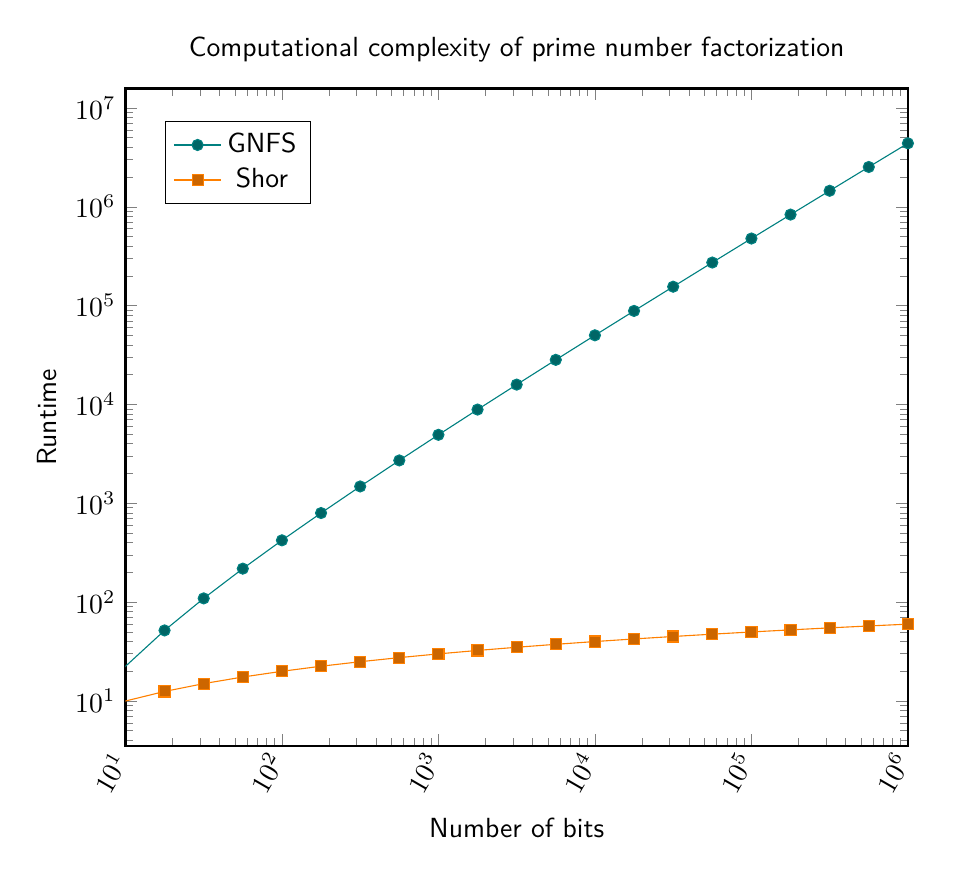
\begin{tikzpicture}
		\begin{loglogaxis}[
			axis line style=thick,
			width=0.95\linewidth,
			title={Computational complexity of prime number factorization},
			xmin=10,
			xmax=1e6,
			xticklabel style={/pgf/number format/1000 sep=, rotate=60, anchor=east},
			xlabel={Number of bits},
			ylabel={Runtime},
			log basis y=10,
			cycle list name=exotic,
			scaled x ticks=false,
			legend style={at={(0.05,0.95)}, anchor=north west,legend columns=1},
		]
			\addplot+[
				domain=1:1e6,
			] {exp(1.9*log2(x^(1/3)*log2(log2(x))^(2/3))};
			\addlegendentry{GNFS}
			\addplot+[
				domain=1:1e6,
			]
			{log2(x^3)};
			\addlegendentry{Shor}
		\end{loglogaxis}
	\end{tikzpicture}
\end{document}